\pagenumbering{arabic}
\setcounter{page}{1}
\section{Warm-up: poor man's approach to Fluid Dynamics}
\begin{quote}
    This simple approach is capable of quite a few important applications!
\end{quote}

\subsection{Leonardo's Law: mass conservation}
\begin{quote}
    What streams into a volume has to stream out again.
\end{quote}

\begin{figure}[h!]
    \centering
    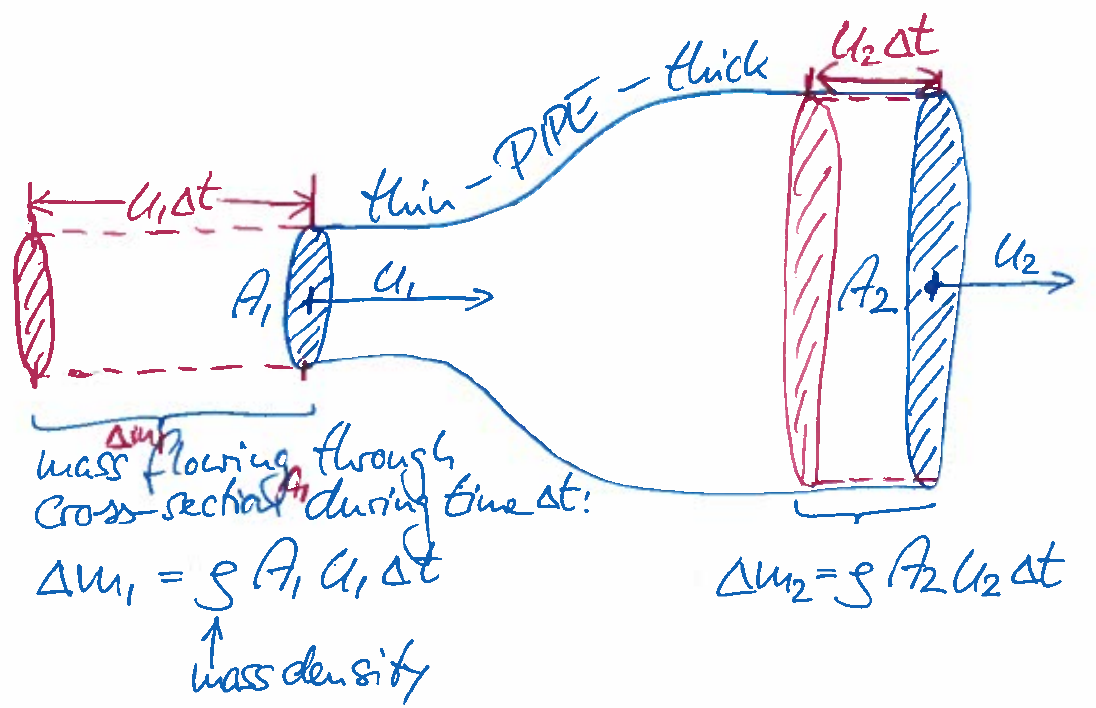
\includegraphics[width=.7\textwidth]{week1/leonardos-law}
    \caption{An illustration of mass conservation.}
    \label{fig:leonardos-law}
\end{figure}

Mass conservation means that the inflow on the left side must equal the outflow on the right side. That is
\begin{align}
    \Delta m_1 &= \Delta m_2\\
    &\Downarrow\notag\\
    \rho A_1 u_1 \Delta t &= \rho A_2 u_2 \Delta t\\
    &\Downarrow\notag\\
    A_1 u_1 &= A_2 u_2 \label{eq:leonardos-law}
\end{align}
Here \eqref{eq:leonardos-law} is known as Leonardo's Law. It has the following properties:
\begin{align}
    A_1 < A_ 2 &\Rightarrow u_1 > u_2\\
    A_1 > A_ 2 &\Rightarrow u_1 < u_2.
    \label{}
\end{align}

\subsubsection{Example 1: why is it always windy on Aarhus Ø?}
\begin{figure}[!h]
    \centering
    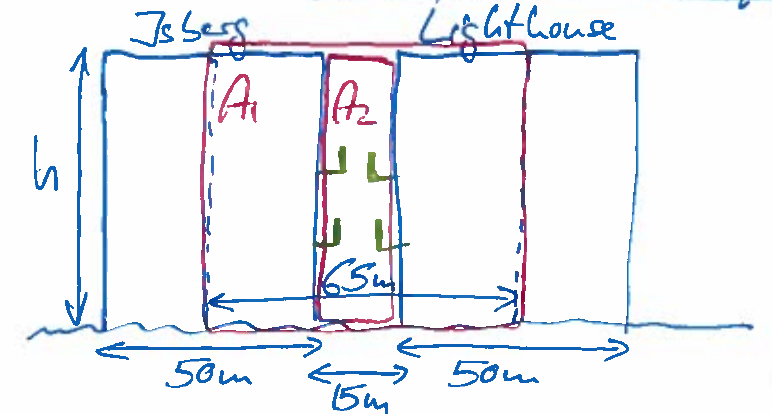
\includegraphics[width=.6\textwidth]{week1/aarhus-oe}
    \caption{The gap between adjacent apartment buildings seen from the side.}
    \label{fig:aarhus-oe}
\end{figure}

In front of the houses:
\begin{equation}
    \Delta m_1 = \rho_\mathrm{air} A_1 u_1 \Delta t
    \label{eq:aarhus-1}
\end{equation}
Between the two houses:
\begin{equation}
    \Delta m_2 = \rho_\mathrm{air} A_2 u_2 \Delta t
    \label{eq:aarhus-2}
\end{equation}
Equating \eqref{eq:aarhus-1} and \eqref{eq:aarhus-2} gives
\begin{equation}
    u_2 = \frac{A_1}{A_2} u_1
    \label{}
\end{equation}
Plugging in "realistic" numbers:
\begin{equation}
    u_2 = \frac{\SI{65}{m}\cdot\mathrm{h}}{\SI{15}{m}\cdot\mathrm{h}} \cdot \SI{10}{m/s} = \SI{43.3}{m/s}
    \label{}
\end{equation}

\begin{description}
    \item[Question:] Why balconies?
    \item[Answer:] Architects are not engineers/physicists!
\end{description}


\subsubsection{Example 2: falling stream of liquid}
\begin{figure}[h!]
    \centering
    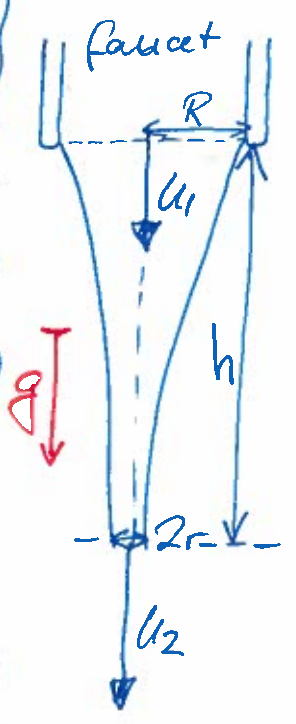
\includegraphics[width=.2\textwidth]{week1/falling-liquid}
    \caption{A stream of falling liquid.}
    \label{fig:falling-liquid}
\end{figure}

We use Leonardo's law:
\begin{equation}
    \pi R^2 u_1 = \pi r^2 u_2
    \label{}
\end{equation}
Energy conservation tells us that the sum of kinetic and potential energy is conserved:
\begin{align}
    \frac{m}{2}u_2^2 &= \frac{m}{2}u_1^2 + mgh\\
    &\Downarrow\notag\\
    u_2^2 &= u_1^2 + 2gh,
    \label{}
\end{align}
where $g=\SI{9.82}{m/S^2}$ is the acceleration of gravity.

\begin{align}
    \frac{r}{R} &= \left(\frac{\pi r^2}{\pi R^2}\right)^\frac{1}{2} = \left(\frac{A_2}{A_1}\right)^\frac{1}{2} = \left(\frac{u_1}{u_2}\right)^\frac{1}{2}\\
    &= \left(\frac{u_1^2}{u_2^2}\right)^\frac{1}{4} = \left(\frac{u_1^2}{u_1^2+2gh}\right)^\frac{1}{4}
    \label{}
\end{align}

\begin{framed}
Remark: The narrowing of a falling stream of liquid holds only for the upper part of the stream. At some height $h$ the stream becomes too thin and drop formation sets in.
\end{framed}


\subsubsection{Example 3: wave energy converter}
\begin{figure}[h!]
    \centering
    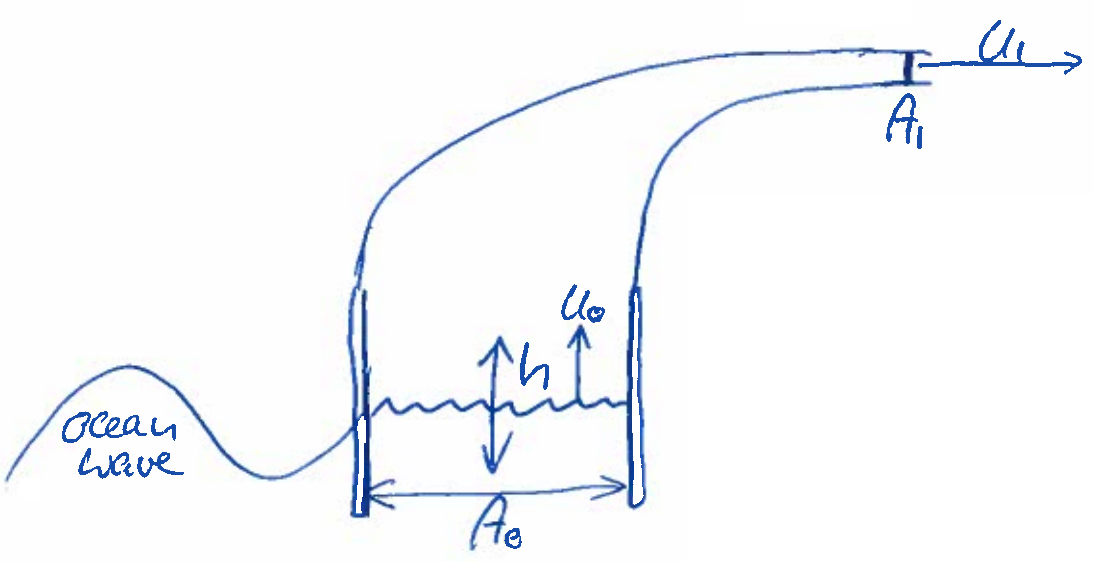
\includegraphics[width=.7\textwidth]{week1/wave-energy}
    \caption{Schematic of a wave energy converter.}
    \label{fig:wave-energy}
\end{figure}
The ocean waves induce an oscillating water surface height, which induces an oscillating air stream. A turbine is placed at the nozzle (with cross-section $A_1\ll A_0$) and extracts power from the moving air stream.

Oscillating height:
\begin{equation}
    h(t) = H \sin \omega t, \qquad \omega = 2\pi f = \frac{2\pi}{T},
    \label{}
\end{equation}
where $f$ is the frequency, $T$ is the oscillating period and $\omega$ is the angular frequency.

\begin{align}
    u_0(t) &= \frac{dh(t)}{dt}\\
    &= H\omega \cos \omega t
    \label{}
\end{align}

\begin{align}
    A_0 u_0(t) &= A_1u_1(t)\\
    &\Downarrow\notag\\
    u_1(t) &= \frac{A_0}{A_1}u_0 \cos \omega t
    \label{}
\end{align}

\begin{equation}
    A_1 \ll A_0 \Rightarrow u_1(t) \gg u_0(t)
    \label{}
\end{equation}


\subsubsection{Example 4: wake flow behind a wind turbine and wind farm optimization}
\begin{figure}[h!]
    \centering
    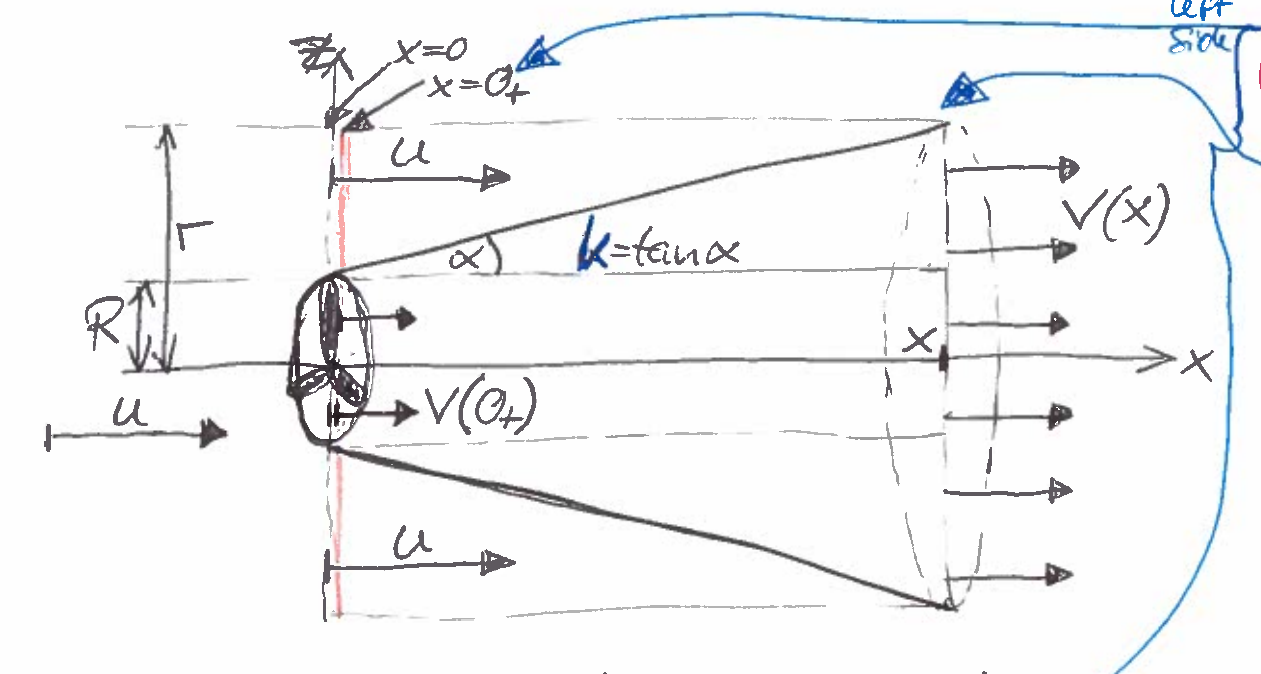
\includegraphics[width=.75\textwidth]{week1/wake-flow}
    \caption{The expanding wake behind a turbine.}
    \label{fig:wake-flow}
\end{figure}
Far-field modeling of a wake flow behind a wind turbine. We use the linear wake expansion:
\begin{equation}
    r = R + kx.
    \label{}
\end{equation}
We use the equation of continuity (Leonardo's law):
\begin{equation}
    \frac{\Delta m}{\Delta t}\biggm\vert_{x=0^+} = \rho\pi R^2v(0^+) + \rho\pi(r^2-R^2)u = \rho\pi r^2 v(x) = \frac{\Delta m}{\Delta t}\biggm\vert_x.
    \label{}
\end{equation}
In words this equation states that the in-flow through the left side of the cylinder is equal to the out-flow through the right side of the cylinder. Rearranging this equation we can get an expression for the wind speed of the wake behind the turbine:
\begin{align}
    v(x) &= \frac{R^2}{r^2}v(0_+)+\frac{r^2-R^2}{r^2}u = u-\frac{R^2}{r^2}\left(u-v(0_+)\right)\\
    &= u \left\{1-\frac{1-\frac{v(0_+)}{u}}{\left(1+\frac{kx}{R}\right)^2}\right\}.
    \label{eq:v-x}
\end{align}
The ratio
\begin{equation}
    q = \frac{v(0_+)}{u}
\end{equation}
is called the axial induction factor.

Consistency checks:
\begin{align}
    \lim_{x\rightarrow 0_+} v(x) &= v(0_+)\\
    \lim_{x\rightarrow\infty} v(x) &= u
\end{align}


\subsubsection*{Betz theory: power produced by a wind turbine}
\begin{figure}[h!]
    \centering
    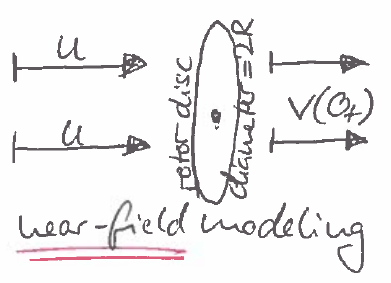
\includegraphics[width=.5\textwidth]{week1/near-field}
    \caption{The velocity deficit caused by the rotor disc.}
    \label{fig:betz}
\end{figure}

A wind turbine extracts kinetic energy out of the wind flow:
\begin{align}
    E_\mathrm{extracted} &= \frac{m}{2} \left(u^2-v^2(0_+)\right)\\
    &= \frac{1}{2}\rho\pi R^2\frac{u+v(0_+)}{2}\Delta t (u^2-v^2(0_+))
    \label{}
\end{align}

\begin{align}
    P_\mathrm{turbine} &= \frac{d E_\mathrm{extracted}}{dt}\\
    &= \frac{\rho\pi R^2 u^3}{2} \left\{\frac{\left(1+q\right)}{2}\left(1-q^2\right)\right\}
    \label{}
\end{align}
The term in front is the kinetic energy contained in the upstream wind (volume). The term within the curly brackets is the efficiency of the wind turbine also called the power coefficient:
\begin{equation}
    C_p = C_p(q) = \frac{\left(1+q\right)}{2}\left(1-q^2\right).
    \label{}
\end{equation}

The maximum efficiency of a turbine can be calculated by requiring
\begin{equation}
\diff{C_p(q)}{q} = \diff{}{q} \left(\half (1+q)(1-q^2)\right) \require 0
\label{eq:power-coefficient}
\end{equation}
This gives the optimal $q$ value
\begin{align}
q &= \frac{1}{3}\\
\leadsto
v(0_+) &= \frac{1}{3}u.
\end{align}

We can then calculate the power coefficient
\begin{equation}
\max_q C_p(q) = C_p(q=\frac{1}{3}) = \frac{16}{27} \approx 0.59.
\end{equation}
This is known as the Betz limit. Real turbines have about $C_p \approx 0.40-0.50$.


\subsubsection{Power optimization of a two-turbine wind farm}
\begin{figure}[h!]
    \centering
    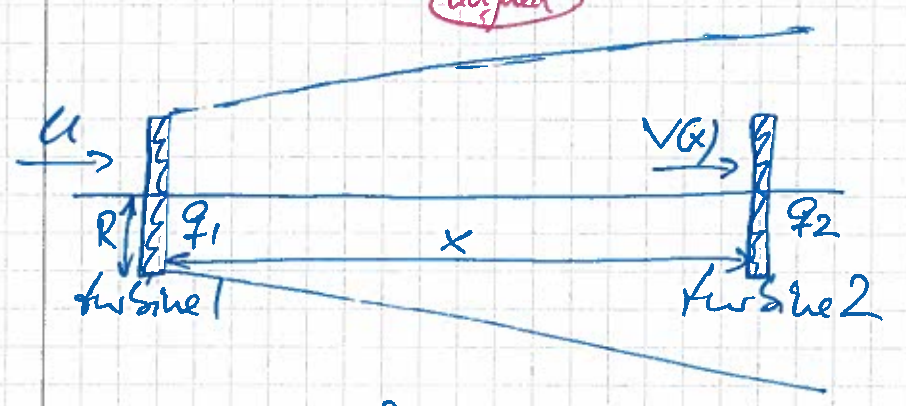
\includegraphics[width=.6\textwidth]{week1/two-turbines}
    \caption{A very simple wind farm consisting of two turbines. The wind is approaching from the left.}
    \label{fig:two-turbines}
\end{figure}

We look at a wind farm with two turbines and a wind direction aligned along the connecting line. The total output of the two turbines is
\begin{equation}
P_{1+2} = \frac{\rho\pi R^2}{2}C_{p_1}(q_1)u^3 + \frac{\rho\pi R^2}{2}C_{p_2}(q_2)v^3(x)
\end{equation}

There are no turbines behind turbine 2, so we configure it to extract the maximum amount of energy from the wind
\begin{equation}
q_2=\frac{1}{3} \Rightarrow C_{p_2}(q_2) = \frac{16}{27}
\end{equation}

Using previous expressions for $C_p(q)$ \eqref{eq:power-coefficient} and $v(x)$ \eqref{eq:v-x} the total output of the two turbines is
\begin{equation}
P_{1+2} = \frac{\rho\pi R^2}{2}u^3 \left\{\half(1+q_1)(1-q_1^2) + \frac{16}{27}\left[1-\frac{1-q_1}{\left(1+\frac{kx}{R}\right)} \right]^3 \right\}
\end{equation}

Similar to before we find the optimal value of $q_1$ by the requirement
\begin{equation}
\diff{P_{1+2}}{q_1} \require 0.
\end{equation}
We fix the values
\begin{align*}
k &= 0.04\\
\frac{x}{R} &= 8.
\end{align*}
The optimal $q$-value for turbine 1 is then
\begin{equation}
q_1 = 0.58 > \frac{1}{3},
\end{equation}
so turbine 1 let's through more wind.

Comparing this result with a $q$-value of $\frac{1}{3}$ gives
\begin{equation}
P_{1+2}(q_1=0.58) = 1.07 \cdot P_{1+2}\left(q_1=\frac{1}{3}\right),
\end{equation}
which is a $7\%$ gain.